\section{Case Study\label{sec:casestudy}: visual exploration of topic modeling in RCloud}

In this section, we present a simple, but real-world example
application currently deployed using RCloud.

This example application is an implementation of LDAVis, a
recently-published method for visualizing large collections of
text. It was specifically designed to enable non-expert users to
explore collections of short text documents using topic modeling and
visualization. Topic modeling~\cite{Blei:2003:LDA} is a standard
technique for text summarization which, although powerful, requires a
certain amount of manual intervention and
interpretation~\cite{Sievert:2014:LAM}.

\begin{figure*}
  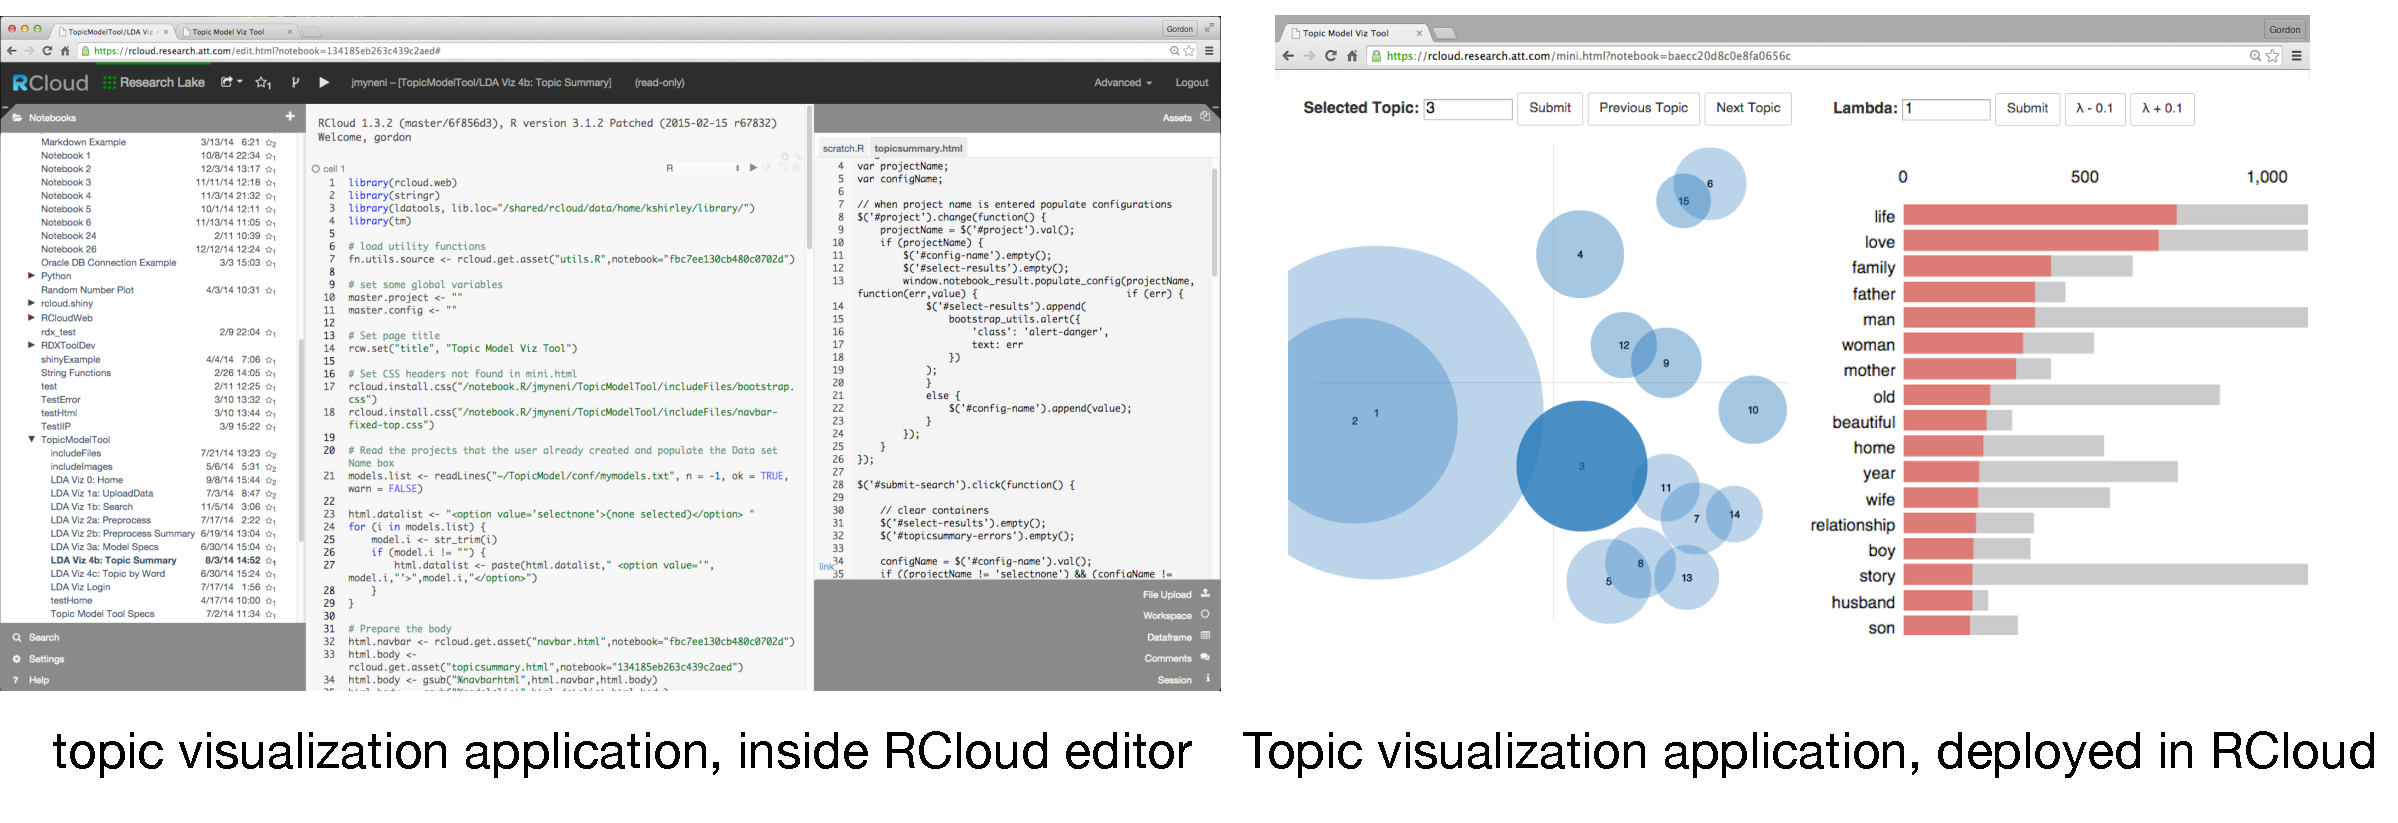
\includegraphics[width=\linewidth]{fig/casestudytext/casestudytext.pdf}
  \caption{\label{fig:textvis}An example application developed and deployed in RCloud.}
\end{figure*}

LDAVis itself was developed by two members of the technical staff at
AT\&T Labs, and originally targeted RStudio's
Shiny~\cite{RStudio:2013:SWA}, a framework for developing R
applications for the web.  While Shiny provides unparalleled ease of
development, discoverability and deployment turn out to be equally
important aspects in the lifecycle of an internal application (see
Section~\ref{sec:interviews}).  On these aspects, RCloud provides a
very simple model: \emph{all developed notebooks are automatically
  deployed}.

LDAVis combines textual analysis, dimensionality reduction, and
interactive visualization. The text analysis is performed via a
combination of an existing R library that fits an LDA model using
Gibbs sampling~\cite{} and some R code written specifically by the
developers. The analysis module is, ultimately, a single R function
that is exposed to the web application via the Javascript-R RPC
mechanism described in Section~\ref{sec:system}; this way, the
analysis is executed remotely on the RCloud servers.

Each textual topic is a probability distribution over the all the
words of the document. In order to expose patterns in the
relationships between the topics, LDAVis employs a combination of
interactive visualization and dimensionality reduction (letting users
choose different measures for the topic distances and different
dimensionality reduction techniques). The dimensionality reduction
algorithms and distance measures are again implemented in R, which
means they are executed on the RCloud servers as well.

The result of the dimensionality reduction is a two-dimensional plot
of the topic space, which can be seen in
Figure~\ref{fig:textvis}. Describe d3 view.

This application is simple, but highlights some of the unique features
of RCloud. While RCloud notebooks allow deployment of R analyses over
the web with no additional effort, RCloud \emph{applications} are more
powerful, and are developed in a combination of Javascript and HTML
for the front end. This requires additional knowledge over Shiny, but
we argue that the RCloud model makes the analysis side simpler for the
analysts (since they simply write the R code in the style they are
used to), and the front-end visualization side simpler for the
front-end developers (since they simply write the Javascript code in
the style \emph{they} are used to). In addition, RCloud applications
inherit the automatic deployment and discoverability features of
regular RCloud notebooks.

%% Text analysis in

%% To illustrate some aspects of RCloud, we present an example notebook
%% for stock price analysis.\footnote{Unfortunately this report could not
%% include production notebooks containing proprietary information.}
%% The example, although simplified, shows key steps in the development
%% and deployment of an application.

%% \begin{figure}
%% 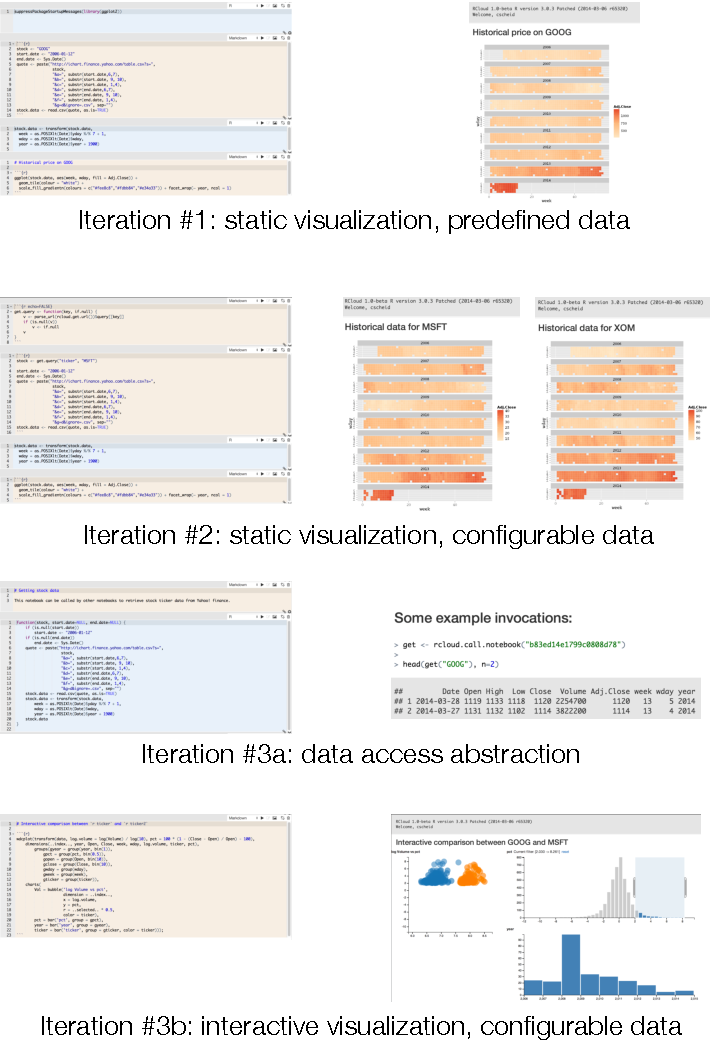
\includegraphics[width=\linewidth]{fig/casestudy1/casestudy1.pdf}
%% \caption{\label{fig:stockvis}Iterations of a stock ticker
%%   visualization, based on an example by Hadley Wickham. A
%%   simple, static visualization of the closing price of a single stock
%%   is progressively developed into a configurable display suitable
%%   for a dashboard, then into an interactive visualization that
%%   compares the volatility and volume of two stocks, and finally
%%   into an API for data access by other RCloud notebooks. The notebooks
%%   in this example can all be loaded as web pages. When a notebook
%%   corresponding to a function call is displayed a web page,
%%   its associated documentation is displayed.}
%% \end{figure}

%% It shows a sequence of visualizations of the performance
%% of financial stocks over several years. The first visualization
%% in this example uses ggplot2 and was written by Hadley Wickham.
%% It reads data provided by Yahoo! Finance as a web service, and shows
%% the price for a single trading symbol.

%% The webpage that produces that visualization includes a link to
%% the underlying source code. From this link, a user can fork the notebook.
%% In the example,a configurable ticker is added, based on the URL of
%% the notebook. The change to the notebook is minor.

%% Next, the notebook author or a collaborator may decide to extend
%% the application to also provide convenient access to the data,
%% apart from its visualization.
%% This is done by creating a notebook that defines a function.
%% That notebook then becomes a \emph{subroutine} for other notebooks.
%% It can be invoked from interactive notebooks, such as dashboards.
%% The data access notebook is version-controlled like other notebooks.

%% Finally, consider the situation where an analyst wants to understand
%% the price dynamics of stocks with respects to other attributes and
%% time ranges. For this, interactive visualization may be very helpful.
%% In our example, the analyst creates an interactive tool with multiple
%% linked views.

%% Demonstrating the integration of R and JavaScript, here the analyst
%% writes an R function that passes the dataframe and description of
%% the charts to the dcplot library.  Simple R expressions
%% are captured as trees to generate JavaScript expressions.
%% The terse chart description language, with sensible defaults inspired by
%% ggplot2, provides a simple yet powerful interface to the grouping
%% and reduction functionality of the well-accepted charting libraries
%% crossfilter, dc.js and d3.js.

% \subsection{Text analysis\label{sec:textvis}}
% Same.

% IMPORTANT: what is unique about RCloud here
% From prototyping to dashboard
% Getting other information from the web
%
